\begin{CJK}{Bg5}{bsmi}

%---------------------------------------------
%	Chapter Preliminaries
%---------------------------------------------

\chapter{Preliminaries}

\section{Digital Signature Algorithm}

Digital signature is a mathematical scheme for demonstrating the authenticity of a digital message or document. 

A digital signature scheme typically consists of three algorithms:

\begin{enumerate}
\item[*] A key generation algorithm that selects a private key uniformly at random from a set of possible private keys. The algorithm outputs the private key and a corresponding public key.
\item[*] A signing algorithm that, given a message and a private key, produces a signature.
\item[*] A signature verifying algorithm that, given a message, public key and a signature, either accepts or rejects the message's claim to authenticity.
\end{enumerate}

Digital signatures can be used to authenticate the source of messages. When ownership of a digital signature secret key is bound to a specific user, a valid signature shows that the message was sent by that user. I take the advantage of this authentication property to replace password. In password-based authentication scheme, the ownership of password is bound to a specific user. 

\section{Android HCE Feature}

Many Android devices which offer NFC functionality also support card emulation feature. In most cases, this feature is achieved by a seperate chip, called \emph{secure element}. The Android system is only provide an interface. Therefore, no Android application can involved in the transaction between secure element and the reader. After the transaction complete, an applications can query the secure element directly to get transaction status and notify users. This is why Tte original NFC card emulaiton functionality also called hardware card emulation.

Because this mechanism needs an extra hardware in devices, most of Android application developers cannot take advantages of card emulation feature. To solve this, Android 4.4 provides an additional method of card emulation, which is not invoved with secure element, called \emph{host-base card emulation}. This method allows Android application can communicate with NFC reader directly, not 

\section{OpenID}

OpenID (OID) is an open standard and decentralized protocol by the non-profit OpenID Foundation that allows users to be authenticated by certain co-operating sites (known as Relying Parties or RP) using a third party service. This eliminates the need for webmasters to provide their own ad hoc systems and allowing users to consolidate their digital identities.[1] In other words, users can log into multiple unrelated websites without having to register with their information over and over again. Fig~\ref{fig:openid-flow} is the overview of OpenID protocol and the user flow.
\begin{figure}
\centering
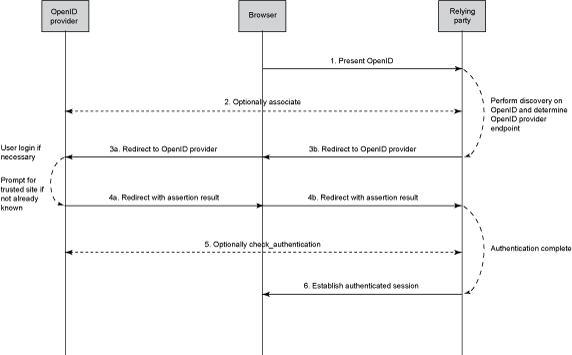
\includegraphics[scale=0.6]{picture/openid-flow.png}
\caption{OpenID overview}
\label{fig:openid-flow}
\end{figure}

\section{Existing Solutions}

Since researchers have studied authentication system for years, there are various of solution now. I selected four kinds of solution, which is related to hardware-token, mobile device and smart card. These features are similar to the scheme I proposed. I describe them briefly in the following section.

\subsection{Token-based scheme}

\subsubsection{SecurID}

SecurID, now known as RSA SecurID, is a mechanism developed by RSA (the Security Division of EMC) for performing two-factor authentication for a user to a network resource. The following paragragh will describe how it works simply.

Each device stored a defferent secret \emph{seed}, and the back-end server also know this seed. In every 60 seconds, SecurID will generate an 6-digit authentication code according to its seed, and display on the screen. If a user authenticating to a network service, he have to enter both a personal identificaiton number and the 6-digit \emph{code at that moment}. The server, which also has a real-time clock and a database of valid tokens with the associated seed records, authenticates a user by computing what number the token is supposed to be showing at that moment in time and checking this against what the user entered.

However, in March 2011 attackers compromised RSA's back-end database of seeds, which allowed them to predict the authentication codes generated by any token at any time. This attack forces RSA Security to replace almost every one of the 40 million SecurID tokens in use.

\subsubsection{YubiKey}

The YubiKey is another authentication hardware token, which shaped like a USB flash drive. It connects to a USB port and identifies itself as a USB keyboard, which allows it to be compatiable to most of computers or laptops with system's native driver. The basic finction of the YubiKey is to generate \emph{One-Time Passwords}. 

When users want to authenticating to a network service by YubiKey, after insert YubiKey into the USB port, users have to touch the YubiKey's OTP generation button. The YubiKey will help users typing a string of printable characters-the concatenation of a fixed \emph{identity string} (replacing the username) and a one-time password (replacingthe password). Then the verify server will check whether the OTP is valid or not, and check the timestamp to resist to the relay-attak.

\subsection{Mobile-device-based scheme}

\subsubsection{Google 2-step}

Two-step verification is a process involving two stages to verify the identity of an entity trying to access services in a computer or in a network. Google was one of the first Internet companies to introduce a two-step verification process. The first authentication step is just like the original scheme, log in with the username and password. The second step required a mobile phone with SMS service. Users must register his phone number to Google. When a user want to start the 2-step authentication, a text message, which including a one-time code, will send to user's mobile phone via SMS. The user have to enter this code on the website in 30 seconds, or this code will be invalid because of timeout.

\subsection{Smart-card-based scheme}

\subsubsection{Song's Smart-card-based Scheme}

In order to address some of the scurity and management problems that occur in traditional password-based authentication protocols, researchin recent decadrs has focused on smart card based password authentication. In 2012, Ronggong Song proposed a new design of smart card based authentication protoccol. In his research, he analyzed the previous propotol proposed by Xu-Zhu-Feng and demonstrated a simple improvement. Futhermore, he designed a new strong smart card based authentication protocol. The following fig~\ref{fig:song-smard-card-scheme} shows that how his new scheme works.

\begin{figure}
\centering
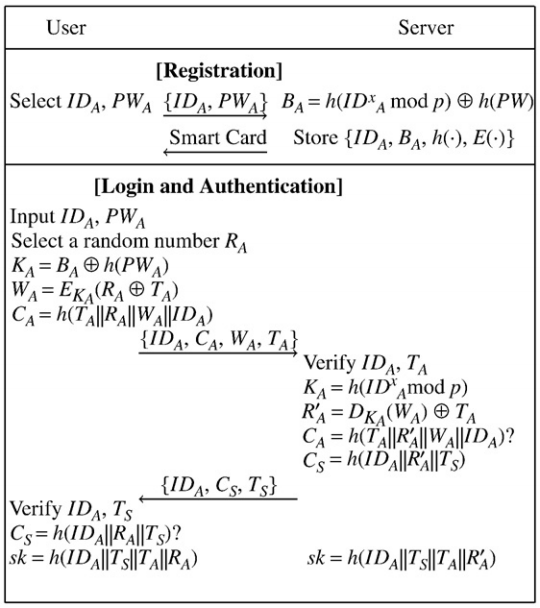
\includegraphics[scale=0.4]{picture/song-smart-card-scheme.png}
\caption{Song's amart cart based authentication scheme}
\label{fig:song-smard-card-scheme}
\end{figure}
\end{CJK}